% MATH 578 HW4
% LUKE WUKMER

\documentclass[10pt]{article}

% note: some of these are extremely useful and i don't remember why :o
%\usepackage{savetrees} % disable custom geometry stuff if you do this
\usepackage{titling}    % contol over title & stuff
\usepackage{amsmath, amsthm, amssymb, amsfonts}
\usepackage{amsxtra, amscd, geometry, graphicx}
\usepackage{endnotes}
\usepackage{cancel}
\usepackage{wrapfig}    %inline figs
\usepackage{bm} %allows fancy stuff like bold greek in math mode
\usepackage{alltt}
\usepackage{enumerate} %more/easier control over lists, also see enumitem
%\usepackage[all,cmtip]{xypic}
\usepackage{mathrsfs}
\usepackage{listings} % code with syntax highlighting etc
\usepackage{caption}
\usepackage[raggedright]{sidecap} % side captions
\usepackage{tabu}     % more customizable tables
%\usepackage{subfigure}
%\usepackage{subcaption}
%\usepackage[pdftex]{hyperref}
%\usepackage[dvips,bookmarks,bookmarksopen,backref,colorlinks,linkcolor={blue},citecolor={blue},urlcolor={blue}](hyperref}

\graphicspath{ {./figs/} }

\usepackage{color}


\definecolor{mygreen}{rgb}{0,0.6,0}
\definecolor{mygray}{rgb}{0.5,0.5,0.5}
\definecolor{mymauve}{rgb}{0.58,0,0.82}

\lstset{ %
basicstyle=\ttfamily,        % the size of the fonts that are used for the code
%breakatwhitespace=false,         % sets if automatic breaks should only happen at whitespace
breaklines=false,                 % sets automatic line breaking
captionpos=t,                    % sets the caption-position to bottom
commentstyle=\color{mygray},    % comment styleh
%  deletekeywords={...},            % if you want to delete keywords from the given language
%  escapeinside={\%*}{*)},          % if you want to add LaTeX within your code
% extendedchars=true,              % lets you use non-ASCII characters; for 8-bits encodings only, does not work with UTF-8
frame=single,                      % adds a frame around the code
%keepspaces=false,                 % keeps spaces in text, useful for keeping indentation of code (possibly needs columns=flexible)
% columns=flexible,
  keywordstyle=\color{blue},       % keyword style
  fontadjust=true,
  language=Python,                 % the language of the code
%  otherkeywords={*,...},           % if you want to add more keywords to the set
  numbers=left,                    % where to put the line-numbers; possible values are (none, left, right)
 numbersep=5pt,                   % how far the line-numbers are from the code
numberstyle=\tiny\color{mygray}, % the style that is used for the line-numbers
%  rulecolor=\color{black},         % if not set, the frame-color may be changed on line-breaks within not-black text (e.g. comments (green here))
showspaces=false,                % show spaces everywhere adding particular underscores; it overrides 'showstringspaces'
showstringspaces=false,          % underline spaces within strings only
%  showtabs=false,                  % show tabs within strings adding particular underscores
%  stepnumber=2,                    % the step between two line-numbers. If it's 1, each line will be numbered
  stringstyle=\color{mymauve},     % string literal style
%  tabsize=2,                      % sets default tabsize to 2 spaces
title=\lstname                   % show the filename of files included with \lstinputlisting; also try caption instead of title
}
% change up the fonts (pick one only)
%\usepackage{times}%
%\usepackage{helvet}%
%\usepackage{palatino}%
%\usepackage{bookman}%
\usepackage{dejavu}


% These are italic.
% \theoremstyle{definition}

% These are normal (i.e. not italic).
\theoremstyle{definition}

%\newtheorem{prob}{Problem}[section]
\newtheorem{prob}{Problem}
\newtheorem*{prob*}{Problem}
\newtheorem*{soln*}{Solution}
\newtheorem{soln}{Solution}


% New Commands: Common Math Symbols
\providecommand{\R}{\mathbb{R}}%
\providecommand{\N}{\mathbb{N}}%
\providecommand{\Z}{{\mathbb{Z}}}%
\providecommand{\sph}{\mathbb{S}}%
\providecommand{\Q}{\mathbb{Q}}%
\providecommand{\C}{{\mathbb{C}}}%
\providecommand{\F}{\mathbb{F}}%
\providecommand{\quat}{\mathbb{H}}%

% haha, i originally forked this template from one provided by my abstract
% algebra TA (back in 2012 or something). probably don't need most of these,
% huh. 

% New Commands: Operators
%\providecommand{\Gal}{\operatorname{Gal}}%
%\providecommand{\GL}{\operatorname{GL}}%
%\providecommand{\card}{\operatorname{card}}%
%\providecommand{\coker}{\operatorname{coker}}%
%\providecommand{\id}{\operatorname{id}}%
%\providecommand{\im}{\operatorname{im}}%
%\providecommand{\diam}{{\rm diam}}%
%\providecommand{\aut}{\operatorname{Aut}}%
%\providecommand{\inn}{\operatorname{Inn}}%
%\providecommand{\out}{{\rm Out}}%
%\providecommand{\End}{{\rm End}}%
%\providecommand{\rad}{{\rm Rad}}%
\providecommand{\rk}{{\rm rank}}%
%\providecommand{\ord}{{\rm ord}}%
%\providecommand{\comp}{{\text{ $\scriptstyle \circ$ }}}%
\providecommand{\cl}[1]{\overline{#1}}%
\providecommand{\tr}{{\sf trace}}%
\providecommand{\spn}{{\rm span}}%

\renewcommand{\tilde}[1]{\widetilde{#1}}%
%\numberwithin{equation}{section}

% i like the squiggly ones more. add as needed

\renewcommand{\Psi}{\varPsi}

\newcommand*\rfrac[2]{{}^{#1}\!/_{#2}}

% a very fancy dot product \ip{f}{g}
\newcommand\ip[2]{ \left\langle {#1} , {#2} \right\rangle }

% "s.t." for math mode
\providecommand{\st}{\text{ s.t. }}

% \norm{f} and such, super useful
\newcommand{\norm}[1]{\left\lVert#1\right\rVert}

% determinant
%\newcommand{\det}[1]{\textsf{det}\left(#1\right)}

% jacobian
\providecommand{\J}{\textsf{J}}

% this makes the spacing between lines of font a little bigger
%\newcommand{\spacing}[1]{\renewcommand{\baselinestretch}{#1}\large\normalsize}
%\spacing{1.2}

\DeclareMathOperator*{\argmin}{arg\,min}
\DeclareMathOperator*{\argmax}{arg\,max}

\newcommand*\mcol[1]{\overset{\big\uparrow}{\underset{\big\downarrow}{#1}}}

% Makes the margin size a little smaller, i gots stuff to say
\geometry{letterpaper,margin=.8in}

% titling stuff (from package titling)
\posttitle{\par\end{center}}
\setlength{\droptitle}{-.5in}
% END PREAMBLE %%%%%%%%%%%%%%%%%%%%%%%%%
%%%%%%%%%%%%%%%%%%%%%%%%%%%%%%%%%%%%%%%%


\begin{document}

\title{Math 578 HW\textsuperscript{\#}4}
\author{Luke Wukmer}
\date{Fall 2016}
\maketitle \thispagestyle{empty} % remove the page number from the first page


%%%% PROBLEM 1

\begin{prob} 
    The entirety of this code is contained in the included single file \texttt{hw4.py}. 
    In the main executing loop (\verb;if __name__ == "__main__": ;),
    various sections have been commented out. Uncomment as desired and run.
    \begin{enumerate}[\bfseries(a)]
        \item
            Cholesky decomposition is performed by the function \texttt{hw4.cholesky}.
            The particular implementation handles sparse matrices as well, and most of the code is
            simply dedicated to choosing the right method based on the data object provided:
            
    \begin{lstlisting}
    def cholesky(A): 
          """ 
          computes the cholesky decomposition for symmetric, positive definite 
          matrices. returns a lower-triangular matril L with positive diagonal 
          entries so that A=LL^T.
          also returns an integer nzl that gives the number of 
          nonzero entries in the Cholesky factor L. 
       
          INPUT: 
       
          A - a positive definite matrix nxn
                (may be np.array or scipy.sparse.spmatrix)
       
          OUTPUT: 
       
          L - the cholesky factor L s.t. A = LL^T 
          nzl - number of nonzero entries in L i.e. where |L_{ij}| > 0 
       
          """ 
           
          if sparse.issparse(A): 
              G = sparse.tril(A) 
              #a sparse matrix that still allows elementwise access 
              G = G.tocsc()
          else: 
              G = np.tril(A) 
              
          n = A.shape[0] 
       
          for k in range(n): 
              G[k:,k] -= G[k:,:k] @ G[k,:k].T 
              G[k:,k] /= np.sqrt(G[k,k]) 
           
          if sparse.issparse(G): 
              nzl = G.count_nonzero() 
          else: 
              nzl = np.count_nonzero(G) 
              
          return G, nzl 
          \end{lstlisting}

          The following suggested sanity check was performed, which yielded the desired result:
    \begin{verbatim}  
In [1]: cholesky(np.array([[2,1,0],[1,2,1],[0,1,2]],dtype='f'))
Out[1]: 
(array([[ 1.41421354,  0.        ,  0.        ],
        [ 0.70710677,  1.2247448 ,  0.        ],
        [ 0.        ,  0.81649655,  1.15470064]], dtype=float32), 5)
    \end{verbatim}

\item
    \begin{figure}
        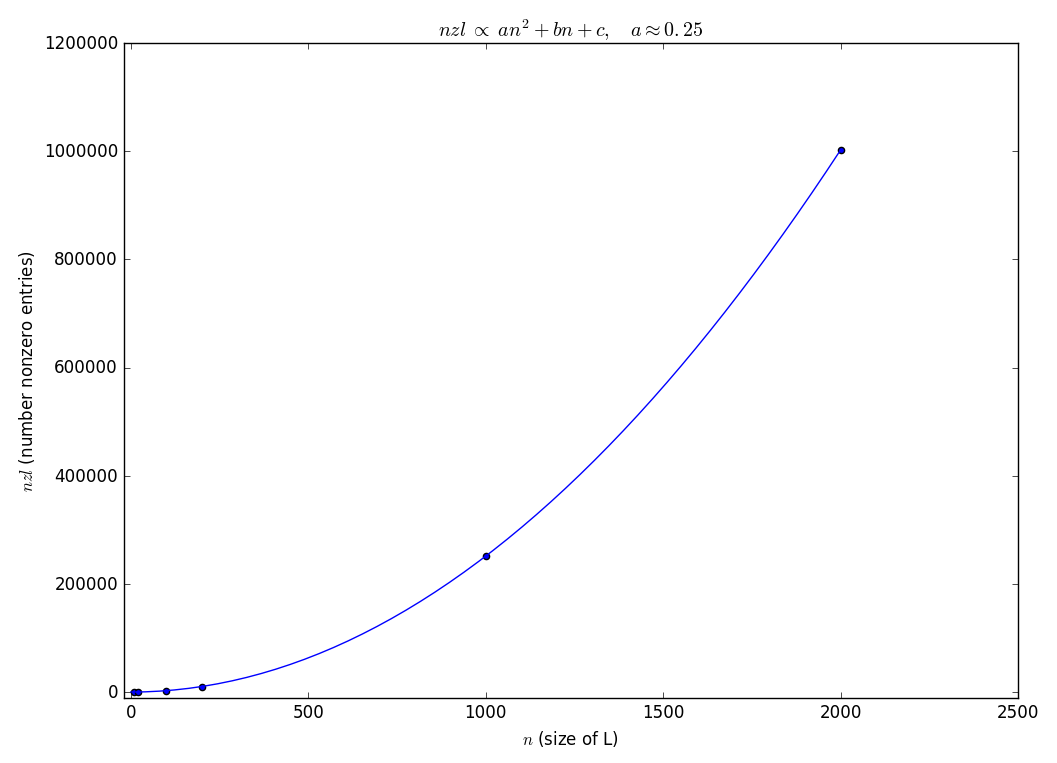
\includegraphics[width=\linewidth]{hw4_1b.png}
        \caption{Relationship between size of system $n$ and number of nonzero elements in Cholesky factor.
        The relationship was found to be quadratic with leading coefficient $a \approx 0.25$.}
    \end{figure}
    Output of spy(L) for $n=2000$:
    \begin{figure}
    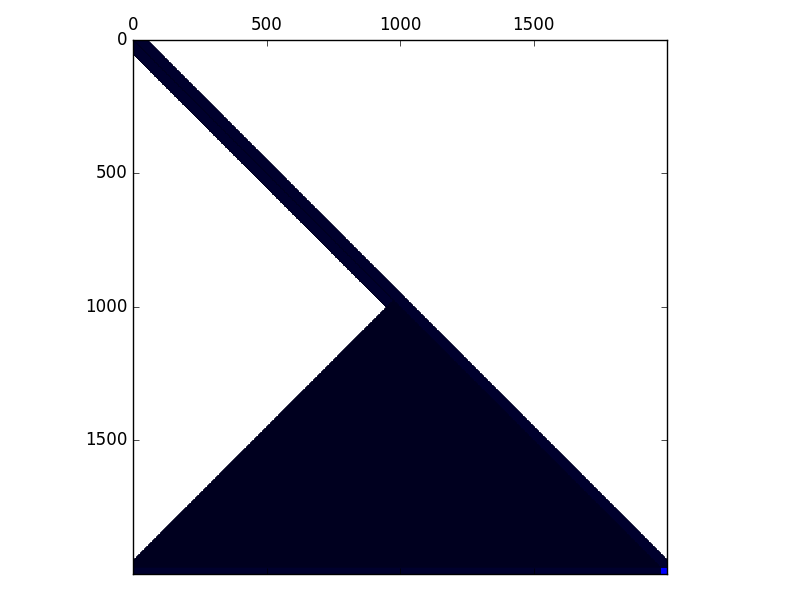
\includegraphics[width=\linewidth]{hw4_spy.png}
    \caption{(\textit{for part (b)}) A visualization of nonzero elements of the cholesky factor $L$ of the matrix A when $n=1000$}
\end{figure}
\item To calculate the size $n$ of system possible to solve with 8GB of memory, we simply use our coefficients we found in part (b) and solve for $n$, given that a 8GB of space can store 8GB $\div$ 8 bytes $\rightarrow$ 1,000,000 nonzero entries. Thus we calculate:
\[
	a n^2 + bn + c = 10^9 \quad \rightarrow \quad 
	\frac{1}{4}n^2 \approx 10^9 \quad \rightarrow \quad \\
	n \approx 63245
\]
\clearpage
\item The multiply function is as follows:
\begin{lstlisting}
def multiply(x, diagonal=None):
    """
    implicitly performs the matrix multiplication Ax
    for the matrix given in (i)

    # test multiply function
    
    n = 60
    x = np.expand_dims(np.random.randn(n),-1)
    A = build_p1(n)

    np.all(np.isclose(A@x,multiply(x))) -> True
    """ 
    if diagonal is None:

        d = 3
    else:
        d = diagonal

    y = np.empty_like(x)
    n = x.size - 1
    n2 = x.size // 2 - 1
    
    # just overwrite the different entries later (ignore 0,n)
    for i in range(1,n):
        y[i] = d*x[i] - x[i+1] - x[i-1] - x[n-i]

    y[0] = d*x[0] - x[1] - x[-1] # first entry
    y[-1] = d*x[-1] - x[-2] - x[0]  # nth (last) entry

    # then overwrite the following:
    y[n2] = d*x[n2] - x[n2+1] - x[n2-1]
    y[n2+1] = d*x[n2+1] - x[n2+2] - x[n2]

    return y 
\end{lstlisting}

\item Conjugate gradient was used to solve the system $Ax=b$ as described. The following iteration numbers and relative errors were reported:
\begin{verbatim}
n		iterations		relative error
10 		3 				1.13492816813e-15
50 		13 				7.26595797191e-12
100 	26 				2.12606603652e-08
5000	1544 			6.25257025384e-07
15000 	4616 			7.0254248905e-07
30000 	9216 			9.29915260829e-07
\end{verbatim}

Clearly, CG does not fare well as the size of the system increases. The conjugate gradient method was implemented as follows:
\clearpage
\begin{lstlisting}
def cg(b=None, n=None, mult=None, tol=1e-6):
    """
    non-preconditioned CG
    initial estimate is b (defaults to normalized ones vector)
    size of system n (can be inferred from b or vice versa)     

    using multiplication method mult
    """

    assert mult is not None

    if b is None:
        try:
            # normalize vector of ones
            b = np.ones((n,1)) / np.sqrt(n)
        except NameError:
            raise Exception('must specify system size or initial guess')
    else:
        n = b.size

    # make sure initial guess is a column vector ala matlab
    if b.ndim == 1:
        b = np.expand_dims(b,-1)
    
    # not sure if explicit copy is needed
    x = np.zeros_like(b)
    r = b.copy()
    p = b.copy()
    
    d = mult(p)

    alpha = np.vdot(r,r) / np.vdot(p,d)

    for iterations in count(1):

        x += alpha*p
        r_new = r - alpha*d

        beta = np.vdot(r_new,r_new) / np.vdot(r,r)

        p = r_new + beta*p

        d = mult(p)
    
        alpha = np.vdot(r_new, r_new) / np.vdot(p,d)
        
        r = r_new

        err = norm(mult(x) - b) / norm(b) 

        #print(iterations, err, sep='\t| ')
        if err <= tol:
            break

    return x, iterations, err
\end{lstlisting}

\item The following iterations and errors were reported for CG when the diagonal elements of the system were perturbed slightly $(3 \rightarrow 3.0001)$   
\begin{verbatim}
n		iterations		relative error
10 		3 				1.88574575416e-15
50 		13 				3.00488927641e-12
100 	26 				9.88035379143e-07
5000 	1519 			8.48965754023e-07
15000 	1835 			9.97779149178e-07
30000 	1797 			9.90061636977e-07
\end{verbatim}

Comparing to the unperturbed system, CG converges faster here. The small perturbation has the effect of lowering the condition number of the matrix.

\item Another multiply function was created for a the system $A = I + BB^T$, and used for conjugate gradient. Implementation as shown:

\begin{lstlisting}
def multiply2(x):
    """
    multiply implicitly by A = I + BB.T
    where B = np.tril(np.ones((n,3))) and n = x.size
    i.e. B = array([[ 1,  0,  0],
                    [ 1,  1,  0],
                    [ 1,  1,  1],
                    [ .   .   .],
                    [ .   .   .],
                    [ .   .   .],
                    [ 1,  1,  1]])

    this faster method is shown by first considering (B.T @ x) itself,
    which yields the 3-vector:
    [ S , S -x[0] , S - x[0] - x[1] ], where S = x.sum()
    """

    S = x.sum()
    
    # do BB.T mult first
    BBx = np.zeros_like(x)
    BBx[0] = S
    BBx[1] = 2*S - x[0]
    BBx[2:] = 3*S - 2*x[0] - x[1]
    
    # now add I part and return
    return x + BBx
    

\end{lstlisting}

Size of system / Iterations / Relative error as shown:
\begin{verbatim}
10000 4 2.06562011245e-15
50000 4 1.82194210335e-14
100000 4 1.15615944448e-13
\end{verbatim}

It's clear that A has at most 4 distinct eigenvalues. Clearly, the matrix $BB^T$ has rank 3 and thus at most 3 distinct eigenvalues. Thus $A = I + BB^T$ has these three plus $0+1$, so 4.
\end{enumerate}
\end{prob}
\end{document}
